%%%%%%%%%%%%%%%%%%%%%%%%%%%%%%%%%%%%%%%%%%%%%%%%%%%%%%%%%%%%%%%%%%%%%%%%%%%%%%%%
%                                                                              %
%                     ELEN4009 - Software Engineering                          %
%                                                                              % %                   Description of Demonstrable Modules                        %
%                                 for                                          %
%         The Online Postgraduate Application Approval System for EIE          %
%                                                                              %
%             Julio Baeta (710066), Nomakhosi Ndebele (671480),                %
%             Ryan Robinson (453764),Timothy Rokebrand (458960)                %
%                                                                              %
%          This LaTeX document was adapted from the IEEE template,             %
%                           which can be found at:                             %
% http://www.ieee.org/conferences_events/conferences/publishing/templates.html %
%                                                                              %
%%%%%%%%%%%%%%%%%%%%%%%%%%%%%%%%%%%%%%%%%%%%%%%%%%%%%%%%%%%%%%%%%%%%%%%%%%%%%%%%

\documentclass[journal,comsoc,onecolumn]{IEEEtran}
\usepackage[T1]{fontenc}
\usepackage{fancyhdr}
\usepackage{graphicx}

%%%%%%%%%%%%%%%%%%%%%%%%%%%%%%%%%%%%%%%%%%%%%%%%%%%%%%%%%%%%%%%%%%%%%%%%%%%%%%%%

\begin{document}
	
%%%%%%%%%%%%%%%%%%%%%%%%%%%%%%%%%%%%%%%%%%%%%%%%%%%%%%%%%%%%%%%%%%%%%%%%%%%%%%%%
	
\title{Description of Demonstrable Modules \\ \vspace{7mm} for \\ \vspace{7mm} The Online Postgraduate Application \\ Approval System for EIE}
	
\author{\vspace{3mm} Julio Baeta (710066), Nomakhosi Ndebele (671480), Ryan Robinson (453764), Timothy Rokebrand (458960)\\ \small \vspace{2mm} School of Electrical \& Information Engineering, University of the Witwatersrand, Private Bag 3, 2050, Johannesburg, South Africa}
	
\markboth{}{}
	
\maketitle

\thispagestyle{empty}
\pagestyle{empty}
	
%%%%%%%%%%%%%%%%%%%%%%%%%%%%%%%%%%%%%%%%%%%%%%%%%%%%%%%%%%%%%%%%%%%%%%%%%%%%%%%%
	
\newpage

\pagestyle{empty}

\section{DESCRIPTION OF DEMONSTRABLE MODULES}
The following document presents a brief description of the modules developed for the system that has been produced thus far. These modules show the basic design of the proposed web page. They also demonstrate the communication between the front-end and back-end modules, which allows for information retrieval from a database.

%%%%%%%%%%%%%%%%%%%%%%%%%%%%%%%%%%%%%%%%%%%%%%%%%%%%%%%%%%%%%%%%%%%%%%%%%%%%%%%%

\section{LOGIN PAGE}
The first page that will be seen by any of the users is the Login page. Although not completely functional at this point in time, this will act as the first line of security when a user logs on to the system.  In future versions, the user will enter their personal details and this information will be used to determine the identity of the user and what level of access they will have to the page. This implies that the database will pass information to the php files and, subsequently, the web page will only display the information relevant to the particular user.
	
\begin{figure}[h]
	\centering
	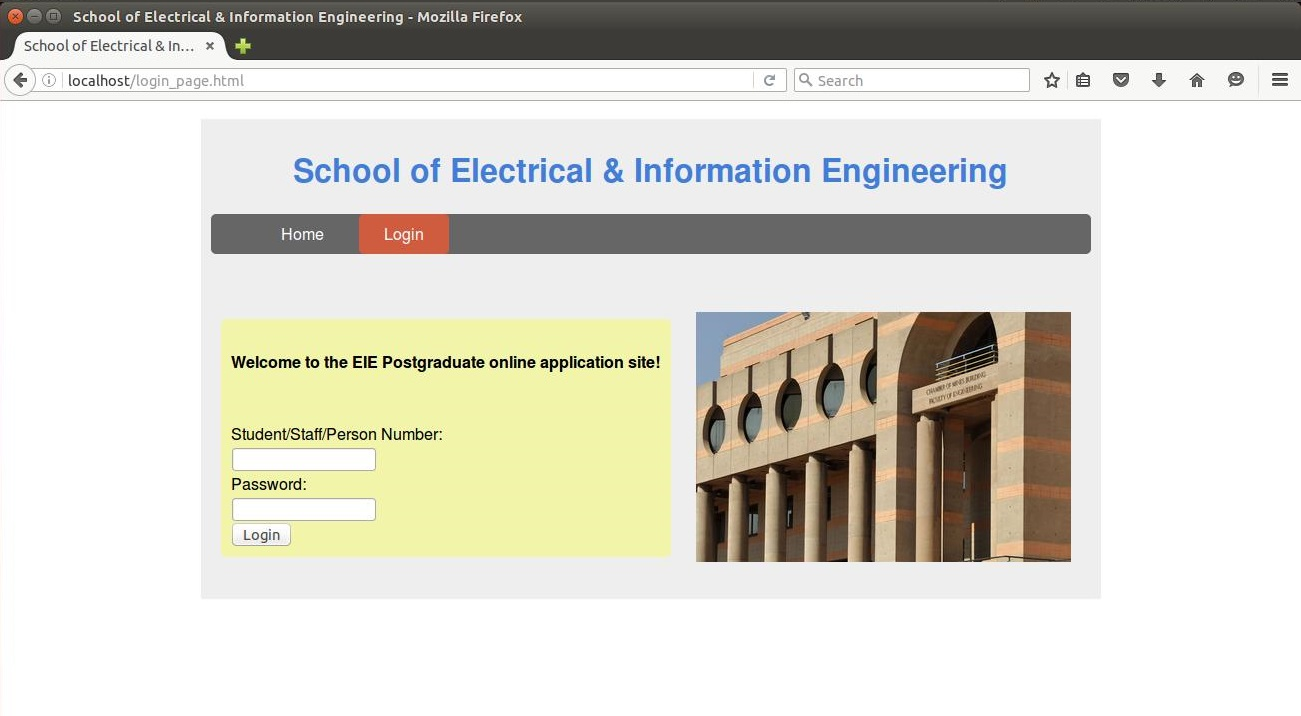
\includegraphics[width=0.7\linewidth]{loginpage}
	\caption{Login Page of the Online Postgraduate Application System}
	\label{fig:loginpage}
\end{figure}

%%%%%%%%%%%%%%%%%%%%%%%%%%%%%%%%%%%%%%%%%%%%%%%%%%%%%%%%%%%%%%%%%%%%%%%%%%%%%%%%

\section{HOME PAGE}
The next page that will be seen by the user is the Home page. Extra information can be added to this page in order to assist the user with understanding the functionality of it and display any additional information that may be of use. The user will be able to navigate back to this page at any time and from any other page. This page welcomes the user and allows the user to navigate to the Applicant List page by clicking, either, on the relevant hyperlink or on the given tab at the top of the screen.
	
\begin{figure}[]
	\centering
	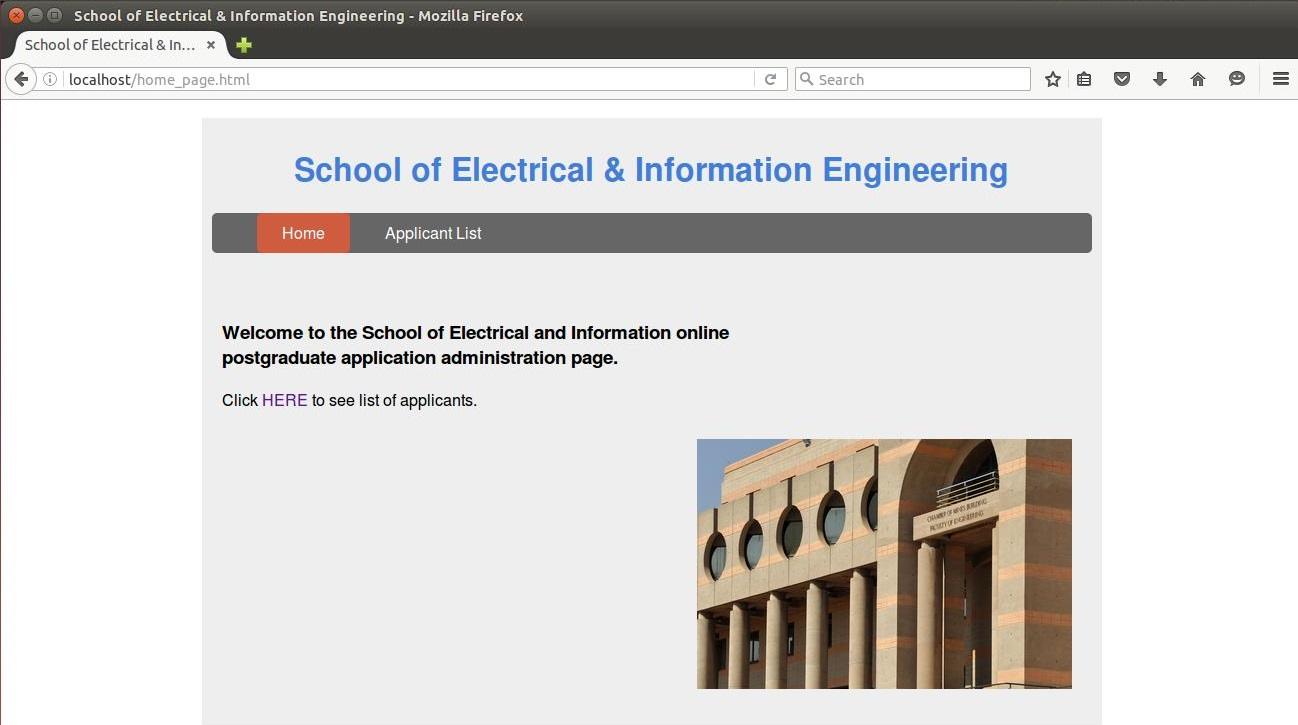
\includegraphics[width=0.7\linewidth]{home}
	\caption{Home Page of the Online Postgraduate Application System}
	\label{fig:home}
\end{figure}
\newpage

%%%%%%%%%%%%%%%%%%%%%%%%%%%%%%%%%%%%%%%%%%%%%%%%%%%%%%%%%%%%%%%%%%%%%%%%%%%%%%%%

\section{APPLICANT LIST}
The Applicant List page shows a list of the potential postgraduate students that are in the process of having their applications processed by the school. The list displays a limited amount of information pertaining to the applicants on this page. The fields include Name and Surname, Supervisor as well as the Program in which they are interested. This list is populated using the created MySQL database. This is achieved by using an unconditional select query, which will retrieve all of the information from the students\_infomation table. In future versions, this information will only be visible to the appropriate supervisors, thus limiting the amount of information that supervisors have access to. 
	
\begin{figure}[h]
	\centering
	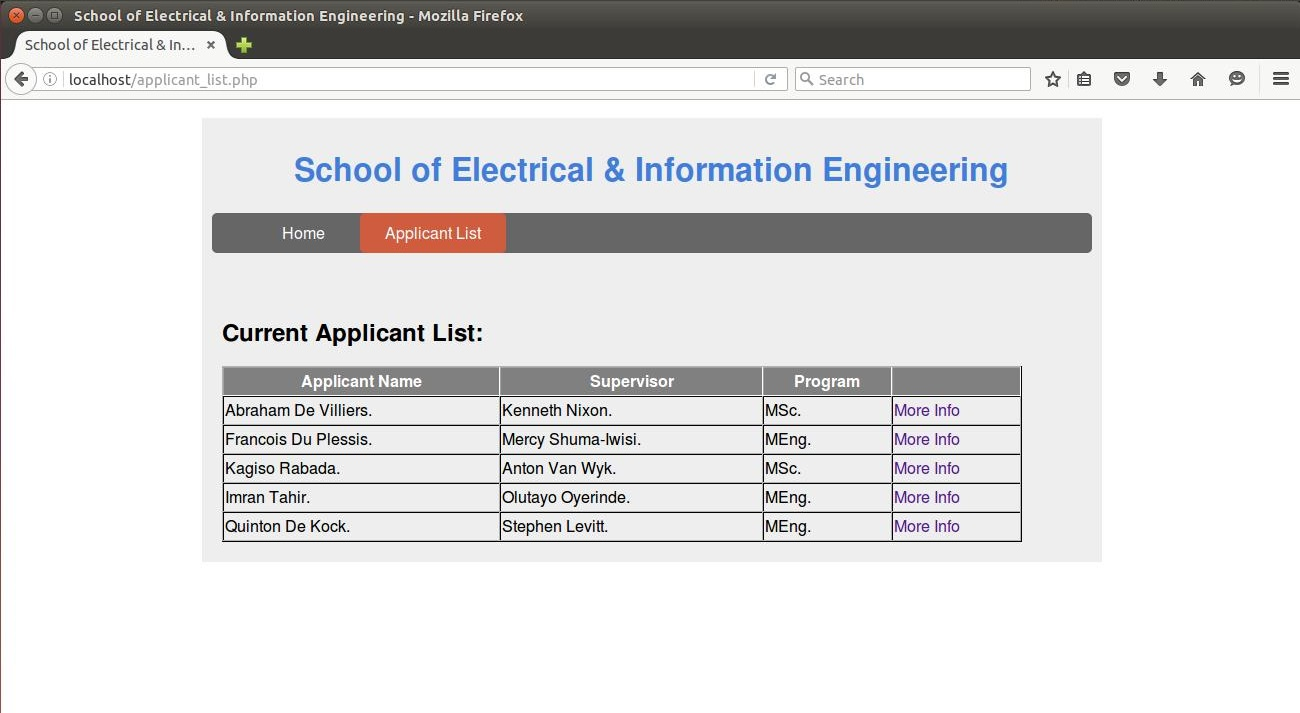
\includegraphics[width=0.7\linewidth]{list}
	\caption{Applicant List found within the Online Postgraduate Application System}
	\label{fig:list}
\end{figure}
	
\hfill \break The student\_information table was created and then populated with insert queries. The resulting table resembled in figure 4.
	
\begin{figure}[h]
	\centering
	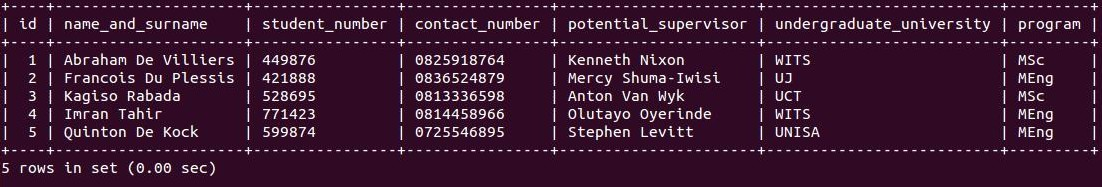
\includegraphics[width=0.7\linewidth]{mysql}
	\caption{Student\_Information Table In MySQL}
	\label{fig:mysql}
\end{figure}

%%%%%%%%%%%%%%%%%%%%%%%%%%%%%%%%%%%%%%%%%%%%%%%%%%%%%%%%%%%%%%%%%%%%%%%%%%%%%%%%

\section{APPLICANT INFORMATION}
When the "More Info" option is selected, a detailed record of the particular applicant's information is displayed. This is achieved by obtaining the relevant postgraduate's identification number within the MySQL database (referred to as 'id' within the database itself), and then passing it to the page though a 'GET' request. The id is then used to modify the select query for the database, such that only the relevant applicant's information is retrieved.
	
\begin{figure}[h]
	\centering
	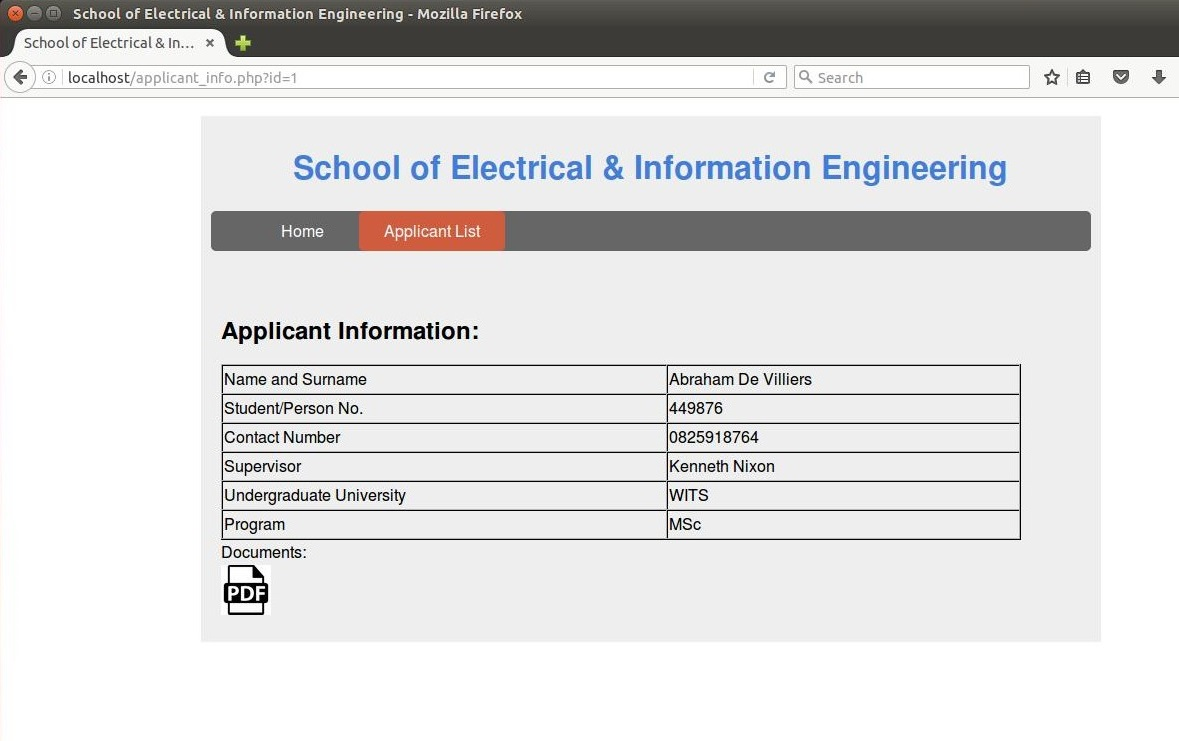
\includegraphics[width=0.7\linewidth]{information}
	\caption{An Applicant's Information Page within the Online Postgraduate Application System}
	\label{fig:information}
\end{figure}

%%%%%%%%%%%%%%%%%%%%%%%%%%%%%%%%%%%%%%%%%%%%%%%%%%%%%%%%%%%%%%%%%%%%%%%%%%%%%%%%

\section{FUTURE DEVELOPMENT}
In future versions, the user will navigate from the Applicant Information page to a Decisions page. Here, the supervisor will be able to approve or reject the application and give comments on their decision. These comments will then be passed to the back-end. \\\\
No security was implemented and this makes the application very risky to use\\\\
Solr was implemented in a limited manner as an extra program needs to be implemented to transfrom rich edit files in this case a pdf into an appropriate format. Once this is acheived the student id could be passed to solr in a select query to obtain the relevent pdf. Solr's full text searching would also allow for students to be corectly located based on terms contained in their pdfs.\\\\

 
	
%%%%%%%%%%%%%%%%%%%%%%%%%%%%%%%%%%%%%%%%%%%%%%%%%%%%%%%%%%%%%%%%%%%%%%%%%%%%%%%%
	
\end{document}

%%%%%%%%%%%%%%%%%%%%%%%%%%%%%%%%%%%%%%%%%%%%%%%%%%%%%%%%%%%%%%%%%%%%%%%%%%%%%%%%